\documentclass[letterpaper]{article}
%\documentclass[letterpaper,10pt]{scrartcl}

\usepackage[utf8]{inputenc}
\usepackage[pass,letterpaper]{geometry}
\usepackage{graphicx}

\title{Non-blocking,In-memory Database\thanks{Sponsor: Dr. Dechev}}
\author{Michael McGee, Robert Medina, Neil Moore, Jason Stavrinaky}
\date{9/18/2015}

\pdfinfo{%
  /Title    (Non-blocking, In-memory Database)
  /Author   (Michael McGee, Robert Medina, Neil Moore, Jason Stavrinaky)
  /Creator  (Neil Moore)
  /Producer ()
  /Subject  (Initial Project Description for COP4934)
  /Keywords ()
}

\begin{document}
  \pagenumbering{gobble}
  \maketitle
  \newpage
  \pagenumbering{arabic}

  \section{Introduction}
  This project's goal is to create a database that utilizes advanced multiprocessor techniques and algorithms to fully utilize modern hardware.
  We will be utilizing the Tervel framework that was developed by Dr. Dechev and his lab that implements multiprocessor-friendly memory management
  as well as various lock-free and wait-free data structures. These data structures will permit us to handle many concurrent transactions without 
  waits or locks.
  
  When we researched how current database systems handle data and their architecture, a typical object-oriented approach does not fit well into the 
  way data flows through a database system. As such, we have decided to take a more functional approach with a focus on transformations on data rather
  than manipulating objects.
  
  \subsection{Broader Impacts}
  An open-source, in-memory and wait-free database would allow for startups or students to experiment with extremely high-frequency applications that
  still need transactional or relational models without dealing with proprietary software such as MemSQL. As the product will be wait-free, scalability 
  with additional hardware should be near-linear as each additional hardware-backed thread allows more concurrent SQL queries to be processed. The 
  applications of such a technology are the same as any other database system, though the speed and scalability of the system lends itself to high-frequency
  and relatively low storage size databases.
  
  \subsection{Motivations}
  \subsubsection{Michael McGee's Motivation}
  My motivation for choosing this project is simply a desire to learn. I have always been interested in database systems as well concurrent programming. Nowhere do these issues more converge than in the project that Dr. Dechev proposed.  
  I hope to gain from this project, a greater understanding of the underlying principles of database system design, as well as discover broader applications for lock-free and wait-free data structures. I know that throughout the course of this project I will learn a great deal and come out as a much improved software developer and computer scientist.  
  \subsubsection{Robert Medina's Motivation}
  My motivation for picking this project is to work a project that I could see other people in a community using on a daily basis. I did not want to work on a program that would be 
  forgotten after it was completed, I want to make a product that has meaning. I think this project has great potential into becoming something that the online community would discuss 
  and possibly can be improved on. I think that databases is a necessary skill for anyone who pursues a career in computer science. The challenge of making a non-blocking database is 
  a great opportunity to showcase my knowledge from the past four years of my education. I look forward into learning about multicore programming, lock-free algorithms, wait-free algorithms,
  and database architecture.
  \subsubsection{Neil Moore's Motivation}
  My motivation for working on this project is to further my knowledge on multiprocessor programming as well as high-performance computing.  
  As hardware vendors put more and more cores into computers, parallelization of algorithms and programs will become much more important than
  single-threaded performance. During my internship, I worked with both GPU compute (OpenCL) and virtualization technologies which exposed me
  to both multiprocessor and system programming. I really enjoyed working on those projects and I think this project will be the next step 
  in my progression as a software engineer and computer scientist.
  \subsubsection{Jason Stavrinaky's Motivation}
  I have always been interested in multiprocessor programming. Considering the future of programming is almost certainly heading towards a
  multiprocessor heavy paradigm, it is an essential skill. Working on a big project involving this is a great opportunity to learn. Not only
  about multiprocessor programming but also memory management. In addition, creating an open source solution to memSQL sounds like an exciting
  challange to undertake while also contributing to the programming community.
  
  \section{Requirements}
  Our deliverable requirements are as follows:
  \begin{itemize}
   \item Able to run SQLLogicTests from the SQLite project.
   \item ANSI SQL Core compliance.
   \item GitHub Page similar to the Tervel framework's.
   \item Source code on the UCF GitHub subdomain.
   \item In-depth documentation on project internals and architecture.
   \item Workshop paper that details new approaches used in database.
  \end{itemize}
  
  \section{Proposed Architecture}
  \centerline{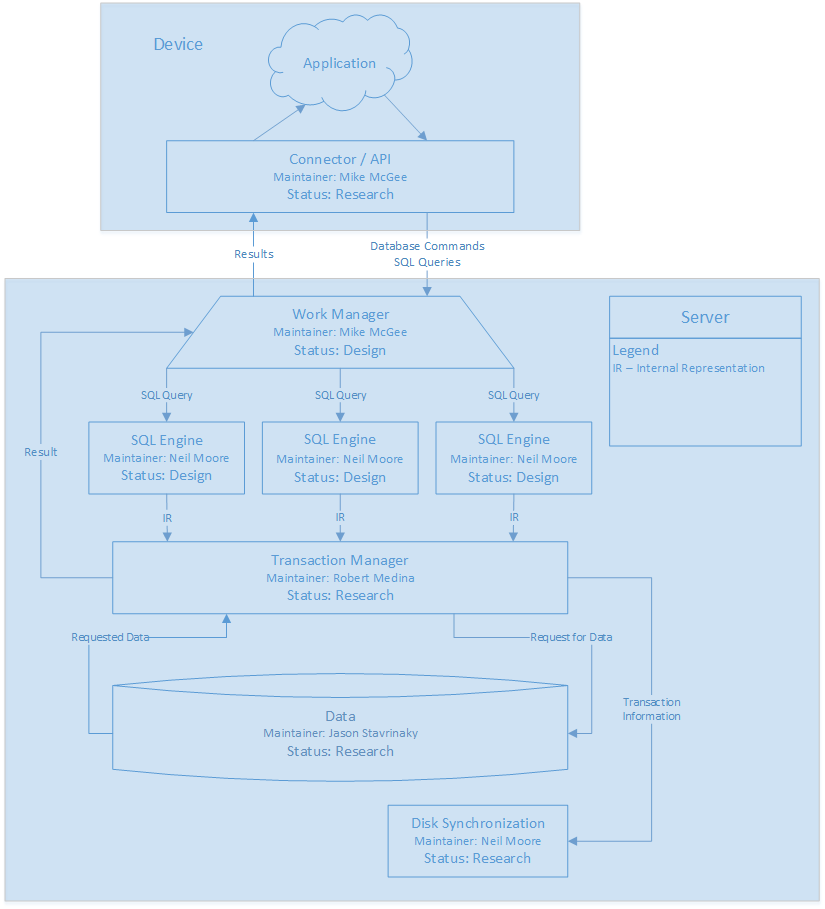
\includegraphics[scale=.75]{OpenMemDbDiagram.png}}
  \subsection{Work Manager}
  The work manager module is the main thread of the system that owns the file descriptor to the the port used by the database as well as managing
  all child threads. It also maintains the connections to the various clients using this database and interacts with their connectors (ODBC, JDBC, etc.),
  as well as with a custom API layer which will be customized
   to our database.
  
  \subsection{SQL Engine}
  This module transforms a SQL query into an internal representation that can then be optimized to our data structures. Is composed of a tokenizer,
  parser, and potentially an optimizer. We're currently looking into open-source implementations of SQL engines to lessen code duplication as well
  as overall effort needed on our part.
  
  \subsection{Transaction Manager}
  The transaction manager provides a central interface to the database objects as well as enforcing the ACID (Atomicity, Consistency, Integrity
  and Durability) guarantees that make up a transaction. This would implement caching techniques as well as snapshot isolation of the
  database. This module would be where most of the interactions between threads occur and as such would utilize the Tervel framework to 
  safely achieve wait-free concurrent access to the database structures.
  
  \section{Financial Concerns}
  Our sponsor is supplying us with a 64-core server that should be sufficient for our development needs. I do not believe any further financial
  support would be required as we are aiming to utilize open-source software and toolkits in our development. An advanced C++ code linter or static
  analyzer is a tool that we may look into acquiring that could require finnancial investment.
  
  \pagebreak
  \section{Project Milestones}
  For this project we're going to utilize the incremental software development process which emphasizes development of small modules concurrently
  with a focus on:
  \begin{itemize}
   \item Communication to understand the objective
   \item Planning (process modeling, data flow)
   \item Development of program modules
   \item Integration and Deployment
  \end{itemize}
  \subsection{Milestone 1 - 10/30/2015}
  \begin{itemize}
   \item Initial documentation.
   \item Workshop paper motivation \& problem statement (half-page each).
   \item Workshop paper related work write-up with comparison to what this project attempts to do (half-page each).
   \item System architecture block diagram.
   \item Basic integration of Tervel into an application along with basic application framework.
  \end{itemize}
  \subsection{Milestone 2 - 12/15/2015}
  \begin{itemize}
   \item Connector implementation that can spawn threads upon SQL queries.
   \item Basic SQL engine that handles parsing and parameterization of queries.
   \item Initial design of API used by applications to access database.
  \end{itemize}
  \subsection{Milestone 3 - 01/30/2016}
  \begin{itemize}
   \item Finalized system architecture.
   \item Rudimentary implementation of the transaction manager.
   \item Preliminary implementation of the disk synchronization service.
   \item Further work on workshop paper.
  \end{itemize}
  \subsection{Milestone 4 - 02/30/2016}
  \begin{itemize}
   \item Finalized API to be used between server and client applications when not using a connector.
   \item First draft of workshop paper.
   \item Implement Atomicity guarantee in the transaction manager.
  \end{itemize}
  \subsection{Milestone 5 - 03/30/2016}
   \begin{itemize}
    \item Implement Consistency and Integrity guarantee in transaction manager.
    \item Another draft of the workshop paper.
    \item Pass SQLLogicTests' core tests.
    \item Exploratory implementation of ODBC driver.
   \end{itemize}
   \subsection{Milestone 6 - 04/13/2016}
   \begin{itemize}
    \item Finalized project with testing. 
    \item Completion of final draft of workshop paper and project presentation.
   \end{itemize}








\end{document}
